\documentclass[]{article}
\usepackage{lmodern}
\usepackage{amssymb,amsmath}
\usepackage{ifxetex,ifluatex}
\usepackage{fixltx2e} % provides \textsubscript
\ifnum 0\ifxetex 1\fi\ifluatex 1\fi=0 % if pdftex
  \usepackage[T1]{fontenc}
  \usepackage[utf8]{inputenc}
\else % if luatex or xelatex
  \ifxetex
    \usepackage{mathspec}
  \else
    \usepackage{fontspec}
  \fi
  \defaultfontfeatures{Ligatures=TeX,Scale=MatchLowercase}
\fi
% use upquote if available, for straight quotes in verbatim environments
\IfFileExists{upquote.sty}{\usepackage{upquote}}{}
% use microtype if available
\IfFileExists{microtype.sty}{%
\usepackage{microtype}
\UseMicrotypeSet[protrusion]{basicmath} % disable protrusion for tt fonts
}{}
\usepackage[margin=1in]{geometry}
\usepackage{hyperref}
\hypersetup{unicode=true,
            pdftitle={Report v2},
            pdfauthor={Xuewan Zhao},
            pdfborder={0 0 0},
            breaklinks=true}
\urlstyle{same}  % don't use monospace font for urls
\usepackage{graphicx,grffile}
\makeatletter
\def\maxwidth{\ifdim\Gin@nat@width>\linewidth\linewidth\else\Gin@nat@width\fi}
\def\maxheight{\ifdim\Gin@nat@height>\textheight\textheight\else\Gin@nat@height\fi}
\makeatother
% Scale images if necessary, so that they will not overflow the page
% margins by default, and it is still possible to overwrite the defaults
% using explicit options in \includegraphics[width, height, ...]{}
\setkeys{Gin}{width=\maxwidth,height=\maxheight,keepaspectratio}
\IfFileExists{parskip.sty}{%
\usepackage{parskip}
}{% else
\setlength{\parindent}{0pt}
\setlength{\parskip}{6pt plus 2pt minus 1pt}
}
\setlength{\emergencystretch}{3em}  % prevent overfull lines
\providecommand{\tightlist}{%
  \setlength{\itemsep}{0pt}\setlength{\parskip}{0pt}}
\setcounter{secnumdepth}{0}
% Redefines (sub)paragraphs to behave more like sections
\ifx\paragraph\undefined\else
\let\oldparagraph\paragraph
\renewcommand{\paragraph}[1]{\oldparagraph{#1}\mbox{}}
\fi
\ifx\subparagraph\undefined\else
\let\oldsubparagraph\subparagraph
\renewcommand{\subparagraph}[1]{\oldsubparagraph{#1}\mbox{}}
\fi

%%% Use protect on footnotes to avoid problems with footnotes in titles
\let\rmarkdownfootnote\footnote%
\def\footnote{\protect\rmarkdownfootnote}

%%% Change title format to be more compact
\usepackage{titling}

% Create subtitle command for use in maketitle
\providecommand{\subtitle}[1]{
  \posttitle{
    \begin{center}\large#1\end{center}
    }
}

\setlength{\droptitle}{-2em}

  \title{Report v2}
    \pretitle{\vspace{\droptitle}\centering\huge}
  \posttitle{\par}
    \author{Xuewan Zhao}
    \preauthor{\centering\large\emph}
  \postauthor{\par}
      \predate{\centering\large\emph}
  \postdate{\par}
    \date{05/12/2019}

\usepackage{graphicx} \usepackage{float} \usepackage{amsmath} \usepackage{threeparttable}

\begin{document}
\maketitle

In this project, we are going to combine fundamental factors and
technical factors to construct portfolios. Fundamental factors are used
to pick more predictable stocks. Then we would use technical factors to
construct forecasting models in trading.

There are two primary methods used to analyze securities and make
investment decisions: fundamental analysis and technical analysis.
Fundamental analysis involves analyzing a company's financial statements
to determine the fair value of the business, while technical analysis
assumes that a security's price already reflects all publicly-available
information and instead focuses on the statistical analysis of price
movements. Technical analysis attempts to understand the market
sentiment behind price trends by looking for patterns and trends rather
than analyzing a security's fundamental attributes.

\hypertarget{introduction}{%
\subsubsection{Introduction}\label{introduction}}

\hypertarget{fundamental-analysis}{%
\paragraph{Fundamental analysis}\label{fundamental-analysis}}

Fundamental analysis determines the health and performance of an
underlying company by looking at key numbers and economic indicators.
The purpose is to identify fundamentally strong companies or industries
and fundamentally weak companies or industries. Investors go long
(purchasing with the expectation that the stock will rise in value) on
the companies that are strong, and short (selling shares that you
believe will drop in value with the expectation of repurchasing when at
a lower price) the companies that are weak. This method of security
analysis is considered to be the opposite of technical analysis, which
forecasts the direction of prices through the analysis of historical
market data, such as price and volume.

For stocks and equity instruments, fundamental analysis uses revenues,
earnings, future growth, return on equity, profit margins, and other
data to determine a company's underlying value and potential for future
growth. In terms of stocks, fundamental analysis focuses on the
financial statements of the company being evaluated. One of the most
famous and successful fundamental analysts is the so-called ``Oracle of
Omaha,'' Warren Buffett, who is well known for successfully employing
fundamental analysis to pick securities.

Corporate fundamental data (anything that might be found on a balance
sheet), is an incredibly useful source of information. Fundamental data
can be used to value companies in pricing models, and one important
analysis is how predictive of future returns each fundamental factor is.

In this project, following fundamental factors are considered. The
factors in this section are discussed in Chapter 5 of Quantitative
Equity Portfolio Management by Qian, Hua and Sorensen, Chapman and Hall,
2007.

\begin{itemize}
\tightlist
\item
  Market Value
\item
  Enterprise Value
\item
  Cash Dividend
\item
  Earnings before Interest, Taxes, Depreciation and Amortization to
  Enterprise Value
\item
  Trailing 12-month earnings to market capitalization
\item
  Book to market capitalization
\item
  Sales to Enterprise Value
\end{itemize}

\hypertarget{technical-analysis}{%
\paragraph{Technical analysis}\label{technical-analysis}}

Technical analysis is a trading discipline employed to evaluate
investments and identify trading opportunities by analyzing statistical
trends gathered from trading activity, such as price movement and
volume. Unlike fundamental analysts, who attempt to evaluate a
security's intrinsic value, technical analysts focus on patterns of
price movements, trading signals and various other analytical charting
tools to evaluate a security's strength or weakness. Technical analysis
can be used on any security with historical trading data.

Across the industry there are hundreds of patterns and signals that have
been developed by researchers to support technical analysis trading.
Numerous types of trading systems are also developed to help them
forecast and trade on price movements. Some indicators are focused
primarily on identifying the current market trend, including support and
resistance areas, while others are focused on determining the strength
of a trend and the likelihood of its continuation. Commonly used
technical indicators and charting patterns include trendlines, channels,
moving averages and momentum indicators.

In general, technical analysts look at the following broad types of
indicators:

\begin{itemize}
\tightlist
\item
  price trends
\item
  moving averages
\item
  volume and momentum indicators
\item
  oscillators
\item
  support and resistance levels
\end{itemize}

\hypertarget{strength-and-weakness}{%
\paragraph{Strength and weakness}\label{strength-and-weakness}}

There are many studies focus only on one of fundamental analysis and
technical analysis. Fundamental analysis serves for long-term value
investment while technical analysis serves for short-term trading.

However, as fundamental analysis focus on long-term performance of the
company, it can't reflect whether we should entry this company at
current price. While technical analysis focus on short-term trading, if
we could choose a fundamental sound instrument, the probability of
success could be improved.

By using both fundamental and technical analysis, the probability of
success could be improved. The idea is to use fundamental analysis to
select sound candidates and use technical analysis to determine the
ideal entry/exit points.

\hypertarget{data}{%
\subsubsection{Data}\label{data}}

\hypertarget{data-source}{%
\paragraph{Data source}\label{data-source}}

Data used in this project contains historical S\&P 500 stocks from
1998/01/01 to 2018/12/31. This time period covers Dot-com bubble, 911
attacks, financial crisis, etc. Thus, our research would be more
reliable and makes it easy to see its performance in extreme situations.

Data source for this project is CRSP/Compustat Merged Database available
from Wharton Research Data Service (WRDS).

\hypertarget{fundamental-factors}{%
\paragraph{Fundamental Factors}\label{fundamental-factors}}

Fundamental factors discussed in this project are based on \emph{Value
Factors Do Not Forecast Returns for S\&P 500 Stocks}.

Fundamental factors are summarized in Table 1.

\begin{table}[H]
\begin{center}
\caption{Value Factor Description}
\label{table1}
\centering
\begin{tabular}{l l}\hline
Value factor & Description \\ \hline
MV & Market Value\\
EV & Enterprise Value\\
CD & Cash Dividend\\
EBITDA2EV & Earnings before Interest, Taxes, Depreciation and Amortization to Enterprise Value\\
E2PFY0 & Trailing 12-month earning to market capitalization\\
B2P & Book to market capitalization\\
S2EV & Sales to Enterprise Value\\
\hline
\end{tabular}
\end{center}
\end{table}

The correlations between the value factors are examined for all stocks
in the S\&P 500 universe throughout the back-test period. In linear
models, a factor may be omitted from the linear regression if it is
highly correlated with another factor. Avoiding highly correlated
factors could also help avoid multi-collinearity, which results in
inaccurate ordinary least squares regression results.

\begin{figure}[H]
\begin{center}
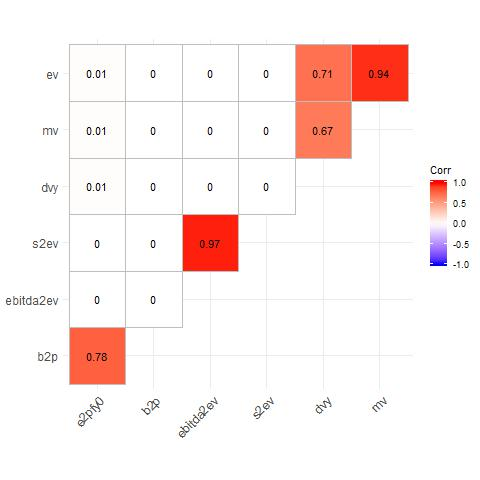
\includegraphics[width=3in]{Lab//CorHeatMap.jpg}
\caption{Factor Correlations}
\label{figure1}
\end{center}
\end{figure}

As we can see from the heat map, two pairs (EV and MV, S2E and
EBITDA2EV) are highly correlated, which makes sense in the stock market.

\begin{figure}[H]
\begin{center}
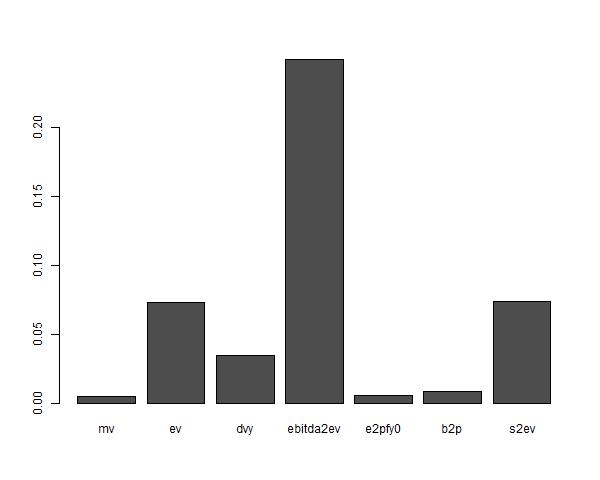
\includegraphics[width=3in]{Lab//NA_in_factors.jpg}
\caption{Factors' NA Percentages}
\label{figure2}
\end{center}
\end{figure}

As a result, we would omit EV in the following analysis in favor of the
MV factor. EBITDA2EV would also be omitted in favor of S2EV.

\hypertarget{sp-500-constitution}{%
\paragraph{S\&P 500 constitution}\label{sp-500-constitution}}

The constitution of S\&P 500 stocks keeps changing, as companies would
enter and exit the stock market. In our model, we are going to use
historical S\&P 500 constitutions, which could help avoid survivor bias.
Some stocks do not exists anymore and the data is missing in
CRSP/Compustat database. However, as we can see below, most stocks are
still recorded and available.

\begin{figure}[H]
\begin{center}
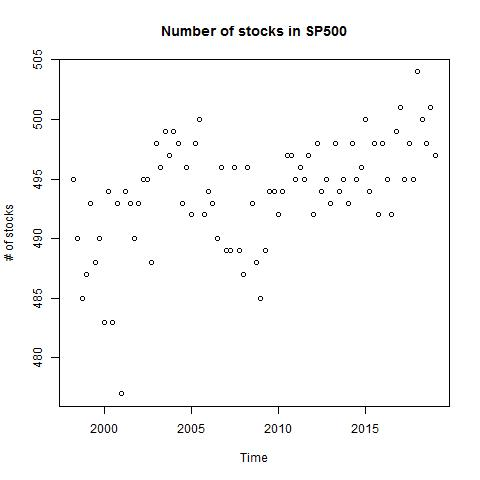
\includegraphics[width=3in]{Lab//Num_of_SP500.jpg}
\caption{Number of S\&P 500 stocks in each quarter}
\label{figure3}
\end{center}
\end{figure}

As we can see, as time goes, the number of available stocks increases.
However, from 2006 to 2009, due to financial crisis, many companies
defaults, which made the number of available stocks during this period
decreases.

\hypertarget{model}{%
\subsubsection{Model}\label{model}}

\hypertarget{fundamental-factor-model}{%
\paragraph{Fundamental factor model}\label{fundamental-factor-model}}

We are going to use fundamental factors to select stocks. There are two
straight ways to select stocks: 1. Pick stocks by ranking the stocks on
the basis of the fundamental factors (one at a time). 2. Pick stocks by
ranking the stocks on the return predicted by a linear model constructed
from the value factors.

After selecting the stocks, there are also two straight ways to trade in
the market: 1. Long the top stocks only. 2. Long the top stocks, short
the bottom stocks which makes us market(dollar) neutral.

Ian L. Kaplan has tested these two ways in \emph{Value Factors Do Not
Forecast Returns for S\&P 500 Stocks}, there are some interesting
conclusions could be referred to here. 1. Multi-factor ranking model
performs better than single factor model. 2. Long/Short Portfolio
performs better than long only portfolio.

Thus, in this project, we are going to use linear multi-factor models to
predict quarterly stock return. Then we would pick top and bottom 20
percent stocks to construct the portfolio. We are going to long the
stocks which we expect would have high return in next quarter and short
the stocks expected to have low returns. Meanwhile, the benchmark would
be the portfolio which invests in all available stocks with equal
weights.

An important thing needs to be noticed is the releasement date of
quarterly fundamental data would be two quarters' later than the quarter
fundamental data belongs to. (i.e.~the fundamental data for March 1998
would not be released before September 1998.)

Assume current time spot is \emph{t}, given previous quarterly
fundamental factors in \emph{t}, we are going to predict the quarterly
return at time \emph{t+1}. However, if we take the lag of information
into consideration, we are actually using data in \emph{t-3} to predict
the quarterly return of \emph{t+1}.

\begin{figure}[H]
\begin{center}
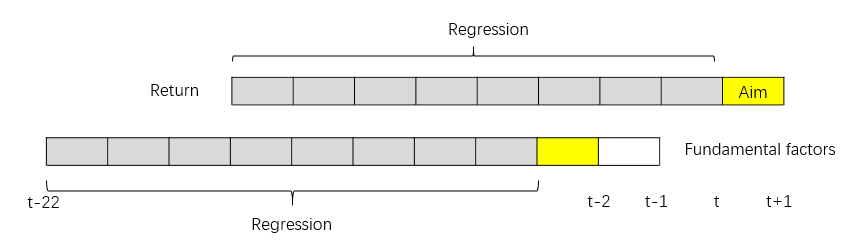
\includegraphics[width=5in]{Lab//RegModel.png}
\caption{Regression model illustration}
\label{figure4}
\end{center}
\end{figure}

As we now have 5 factors, math illustration of regression would be:

\[
r_{t+1} = \beta_0 + \beta_1f_{t,1} + \beta_2f_{t,2} + \beta_3f_{t,3} + \beta_4f_{t,4} + \beta_5f_{t,5} + \epsilon_t
\]

To make our model estimations updated to most recent situation for each
time, we are going to use multiple linear regression with rolling window
to determine the estimations at time t.

\[
\left(\begin{array}{c}
r_t\\
r_{t-1}\\
\vdots \\
r_{t_19}
\end{array}\right)=
\left(\begin{array}{cccc}
1 & f_{t-1,1} & \cdots & f_{t-1,5}\\
\vdots & \vdots & \ddots & \vdots \\
1 & f_{t-20,1} & \cdots & f_{t-20,5}
\end{array}\right)
\left(\begin{array}{c}
\beta_0\\
\beta_1\\
\vdots \\
\beta_5
\end{array}\right)+
\left(\begin{array}{c}
\epsilon_{t-1}\\
\epsilon_{t-2}\\
\vdots \\
\epsilon_{t-20}
\end{array}\right)
\]

After determine the estimations at time t using last 20 quarters' (5
year) data, we are going to forecast the return during time period
\emph{t} to \emph{t+1}.

To be continued: OLS vs Robust OLS vs WLS

\hypertarget{technical-factor-model}{%
\paragraph{Technical factor model}\label{technical-factor-model}}

In this factor model, only technical factors would be used to predict
the daily log return of stocks.

\begin{table}[H]
\begin{threeparttable}  
\begin{center}
\caption{Technical Factors}
\label{table2}
\centering
\begin{tabular}{c c c}\hline 
Symbol & Variable & Function\\ \hline 
\\
SMA20 & Simple moving average in 20 days & \(\displaystyle \frac{C_t+\cdots+C_{t-n+1}}{n}\)\\[12pt]
EMA20 & Exponentially weighted moving average in 20 days & $kC_t+(1-k)EMA_{t-1}$\\[12pt]
Vol & Volume & $V_t$\\[12pt]
MMT & Momentum & $C_t-C_{t-n}$\\[12pt]
SKP & Stochastic K\% & \(\displaystyle 100\frac{C_t-LL_{t,t-n}}{HH_{t,t-n}-LL_{t,t-n}}\)\\[12pt]
SDP & Stochastic D\% & \(\displaystyle \frac{\sum_{i=0}^{n-1} SKP_{t-i}}{n}\)\\[12pt]
RSI & Relative Strength Index & \(\displaystyle 100-\frac{100}{1+(\sum_{i=0}^{n-1} Up_{t-i})/(\sum_{i=0}^{n-1} Dw_{t-i})}\)\\[18pt]
MACD & Moving Average Convergence Divergence & $MA(m_1)-MA(m_2)$\\[12pt]
LWR & Larry William\'s R\% & \(\displaystyle \frac{H_{t-n}-C_{t-n}}{H_{t-n}-L_{t-n}}\)\\[14pt]
ADI & Accumulation Distribution Oscillator & \(\displaystyle ADI_{t-1}+\frac{2C_t-H_t-L_t}{H_t-L_t}V_t\)\\[12pt]
CCI & Commodity Channel Index & \(\displaystyle \frac{(H_t+L_t+C_t)-3SMA_t}{0.045AD_t}\)\\[12pt]
\hline
\end{tabular}
\begin{tablenotes}
\small
\item C: Close price; H: High price; L: Low price; n: Look-back period; HH: Highest high price; LL: Lowest low price; AD: Average deviation.
\end{tablenotes}
\end{center}
\end{threeparttable}
\end{table}

To be continued: Try to use return as weight? Or equal weighted?
artificial neural network, support vector machines with polynomial and
radial basis function kernels.

\hypertarget{stock-screening}{%
\subsubsection{Stock screening}\label{stock-screening}}

In this part, we are going to select 40 stocks which have best/worst
performance according to our fundamental factor model and examine the
performance of our model.

Survivorship bias is the tendency to view the performance of existing
investments in the market as a representative comprehensive sample.
Survivorship bias can result in the overestimation of historical
performance and general attributes of an investment. Survivorship bias
may also be known as ``survivor bias.''

In this paper, as the constitution of S\&P 500 is changing (Some
companies would exit the market), there would be survivor bias if we use
all stocks in the constitution as our stock pool. To avoid survivor
bias, we are going to randomly select 2/3 available stocks as our base
stock pool in each quarter.

In this part, we'll use 1998-2008 data as in-sample period and 2009-2018
data as out-of-sample period. As financial crisis happened during
2007-2008, we are not going to separate these two years.

Survivorship bias is the tendency to view the performance of existing
investments in the market as a representative comprehensive sample.
Survivorship bias can result in the overestimation of historical
performance and general attributes of an investment. Survivorship bias
may also be known as ``survivor bias.''

\textbf{In sample test:}

Due to the property of our model, we need at least 5 years' data
lookback period. Thus, the earliest quarter could be predicted is first
quarter of 2003.

\begin{figure}[H]
\begin{center}
\includegraphics[width=5in]{Lab//In_sample_qtrly_return.jpg}
\caption{In sample quarterly return}
\label{figure5}
\end{center}
\end{figure}

\begin{figure}[H]
\begin{center}
\includegraphics[width=5in]{Lab//In_sample_cumu_return.jpg}
\caption{In sample cumulative return}
\label{figure6}
\end{center}
\end{figure}

It's interesting to see that the performance of our model always goes
opposite with the benchmark. This observation is also supported by
R-squared:

\begin{figure}[H]
\begin{center}
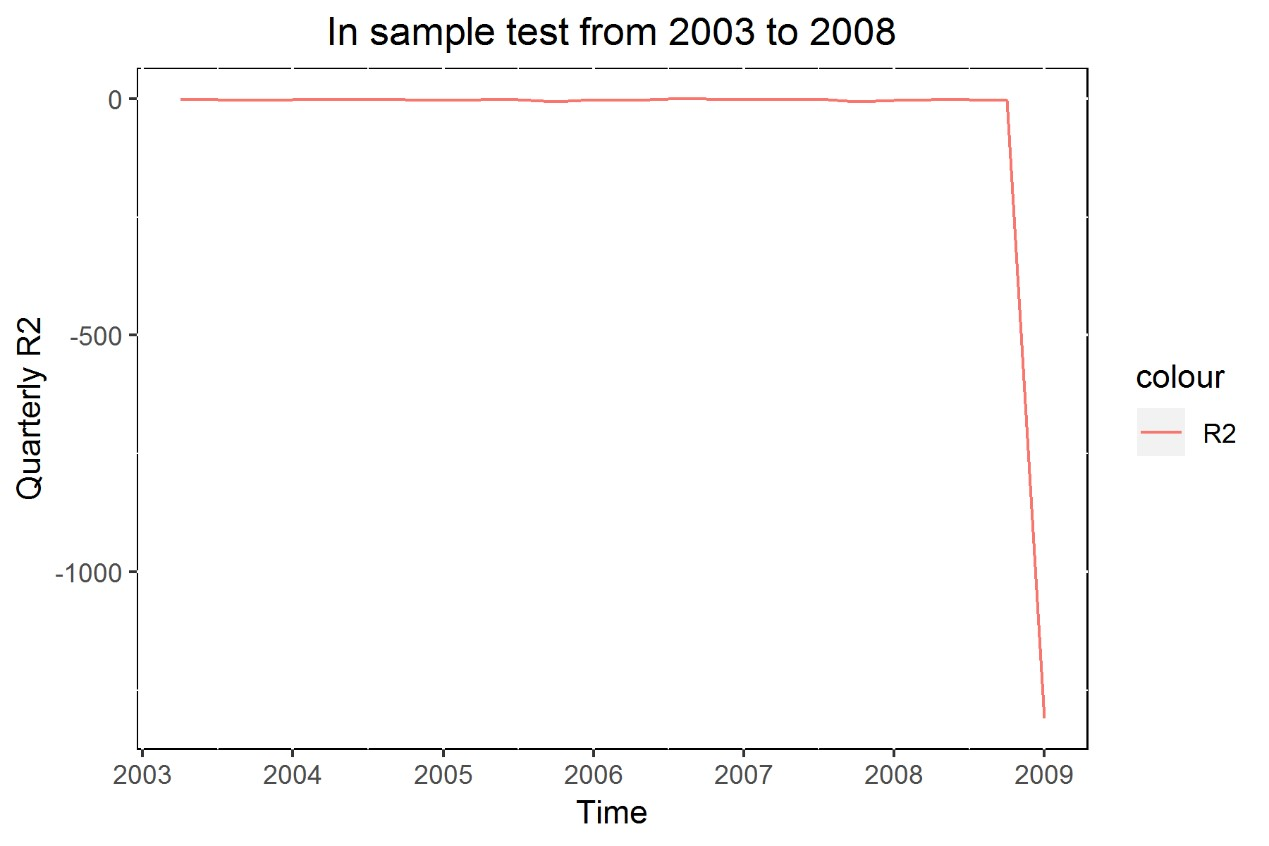
\includegraphics[width=5in]{Lab//In_sample_r2.jpg}
\caption{In sample R-squared}
\label{figure7}
\end{center}
\end{figure}

We can see, the r-square for each quarter is negative. Even that's the
case, we can take advantage of our in-sample test. In out-of-sample
test, we are going to assume the stocks would tend to perform in
opposite direction with our prediction. Then we would do the opposite
trading: long stocks with low expected returns and short stocks with
high expected returns.

Another thing needs to be mentioned is: as we can see from results, the
market volatiles during and after financial crisis period.

There are some possible reasons why our prediction goes in the opposite
direction against real situation:

\begin{enumerate}
\def\labelenumi{\arabic{enumi}.}
\item
  Information already been realized in market. As we are trying to
  predict the return two quarters' later, although the official reports
  are just released, the information in official reports may have
  already been acknowledged by the market through observations or other
  methods. Thus, the price movements indicated by previous quarterly
  reports are already realized.
\item
  The price movements are mean reverting. This is consistent with the
  speculation above. This would explain why our r-square is always
  negative.
\end{enumerate}

\textbf{Verification:} We can verify our speculations by: 1. Use the
most recent fundamental factors to predict the return in next quarter,
i.e., ignoring the `two quarter's lateness' in real world.

\begin{figure}[H]
\begin{center}
\includegraphics[width=5in]{Lab//In_sample_qtrly_return_v1.jpg}
\caption{In sample cumulative return v1}
\label{figure8}
\end{center}
\end{figure}

\begin{figure}[H]
\begin{center}
\includegraphics[width=5in]{Lab//In_sample_cumu_return_v1.jpg}
\caption{In sample cumulative return v1}
\label{figure9}
\end{center}
\end{figure}

Once we changed our trading method and re-test the in-sample period,
we'll see this model performs pretty well.

\begin{enumerate}
\def\labelenumi{\arabic{enumi}.}
\setcounter{enumi}{1}
\tightlist
\item
  Test the mean reverting property of stock returns.
\end{enumerate}

We do the augmented Dickey--Fuller test (ADF) to test the mean reversion
property of stock returns. In this part, we collect the p-value of ADF
statistics. Once p-value is smaller than 0.05, we recognize this stock
as mean reverting. As there are different lags, we would present the
percentage of mean reverting stocks with different each lag terms.

\begin{figure}[H]
\begin{center}
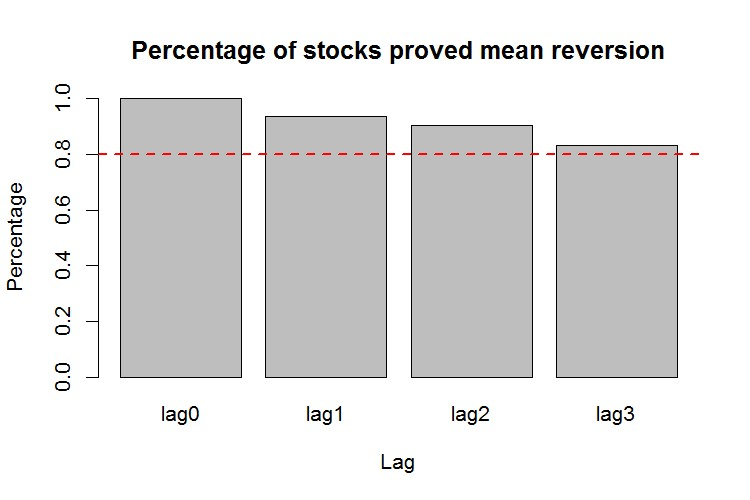
\includegraphics[width=5in]{Lab//mean_rev_pctg.jpg}
\caption{Percentage of mean reverting stocks}
\label{figure10}
\end{center}
\end{figure}

\textbf{Out of sample test:}

Now we apply our model to out-of-sample period and check its
performance.

\begin{figure}[H]
\begin{center}
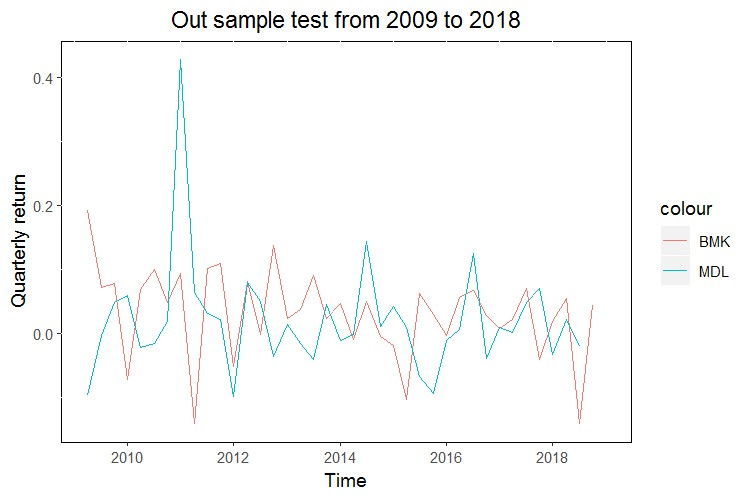
\includegraphics[width=5in]{Lab//Out_sample_qtrly_return.jpg}
\caption{In sample quarterly return}
\label{figure11}
\end{center}
\end{figure}

\begin{figure}[H]
\begin{center}
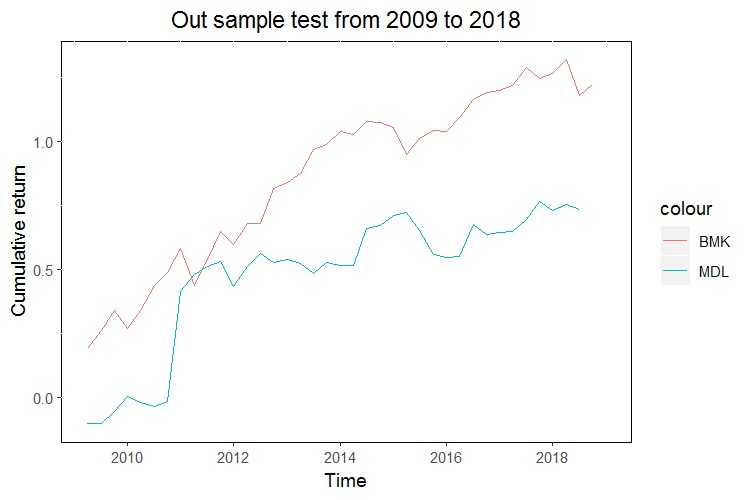
\includegraphics[width=5in]{Lab//Out_sample_cumu_return.jpg}
\caption{In sample cumulative return}
\label{figure12}
\end{center}
\end{figure}

\begin{figure}[H]
\begin{center}
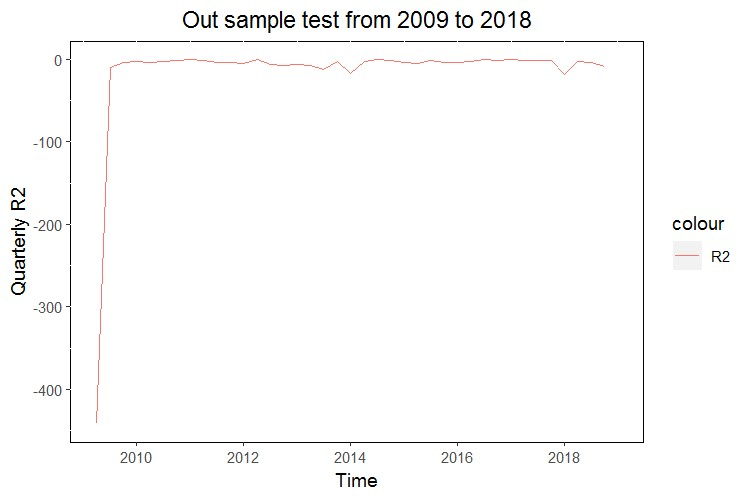
\includegraphics[width=5in]{Lab//Out_sample_r2.jpg}
\caption{In sample R-squared}
\label{figure13}
\end{center}
\end{figure}

We can see that our portfolio generates less return, while its
performance is less volatile. We can check the information ratio of our
model and the benchmark portfolio.

\begin{table}[H]
\begin{center}
\caption{Comparasion of information ratio}
\label{table1}
\centering
\begin{tabular}{l l l}\hline
Information Ratio & Benchmark   & Model \\ \hline
In sample (2003-2008) & 0.09236724 & 0.3858518 \\
Out sample (2009-2018) & 0.3303293 & 0.2384175 \\
\hline
\end{tabular}
\end{center}
\end{table}

If we refer to the 10-year performance of portfolios in the market, we
can see our model beats 75\% portfolios in the market. However, it can't
beat benchmark portfolio during out-of-sample period. There may be some
possible reasons:

\begin{enumerate}
\def\labelenumi{\arabic{enumi}.}
\item
  In bull market, most stocks are increasing, only pick top/bottom
  stocks are not suitable. For example, once we predict all stocks'
  price would increase, we would not short any stocks.
\item
  This strategy suits in bear market, i.e., it would be with low risk
  meanwhile with low return. This speculation is consistent with its low
  volatility property, at the same time its information ratio is still
  good.
\end{enumerate}

\textbf{Verification:}

We can verify our speculations by: 1. Verify the performance of stocks
during 2009-2018.

\begin{figure}[H]
\begin{center}
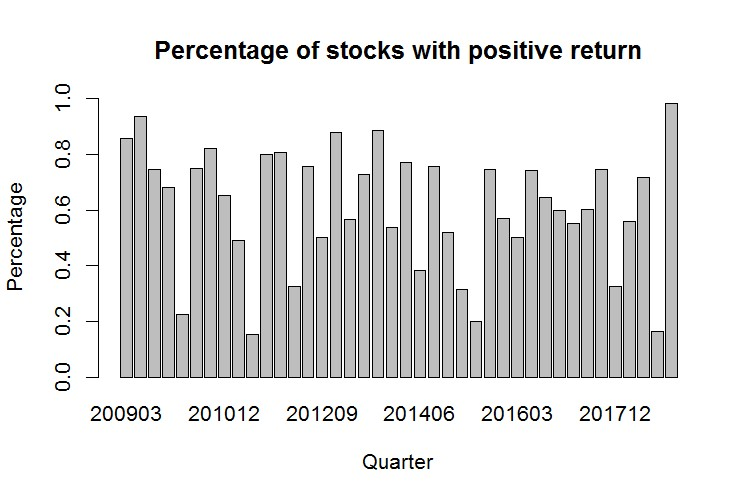
\includegraphics[width=5in]{Lab//Pos_stock_ptg.jpg}
\caption{In sample R-squared}
\label{figure14}
\end{center}
\end{figure}

\begin{figure}[H]
\begin{center}
\includegraphics[width=5in]{Lab//Pos_stock_ptg_dist.jpg}
\caption{In sample R-squared}
\label{figure15}
\end{center}
\end{figure}

We can see clearly from the distribution of the percentage of stocks
which have positive return in each quarter, from 2009 to 2018, the whole
market status should belong to bull market, which consists with our
speculation.

\hypertarget{portfolio-trading}{%
\subsubsection{Portfolio trading}\label{portfolio-trading}}

As we have tested the performance of the strategy based on fundamental
factors, we are going to test the performance of strategies based on
technical factors. In this part, we will base on the results from above
parts, i.e., we will use stocks selected by fundamental analysis.

We are going to use technical factors to predict daily return of stocks.
Once we predict certain stock would have positive return, we will long
this stock, vice versa.

\(\displaystyle r_{t+1} = \beta_t + \beta_oopen_t+\beta_cclose_t+\beta_llow_t+\beta_hhigh_t+\beta_vvol_t+\beta_ssma_t+\beta_eema_t+\beta_mmmt_t+\beta_{fk}fastK_t+\beta_{fd}fastD_t + \beta_{sd}slowD_t+\beta_rrsi_t+\beta_{macd}macd_t+\beta_{lwr}lwr_t+\beta_aadi_t+\beta_ccci_t\)

To analyze the performance of technical factor model itself, we will
compare the portfolio return with another benchmark portfolio. Benchmark
portfolio would only long or short stocks in each quarter, which means
there won't be any daily adjustment on stock holding during a certain
quarter period.

We test this model on the time period 2009 to 2018.

\begin{figure}[H]
\begin{center}
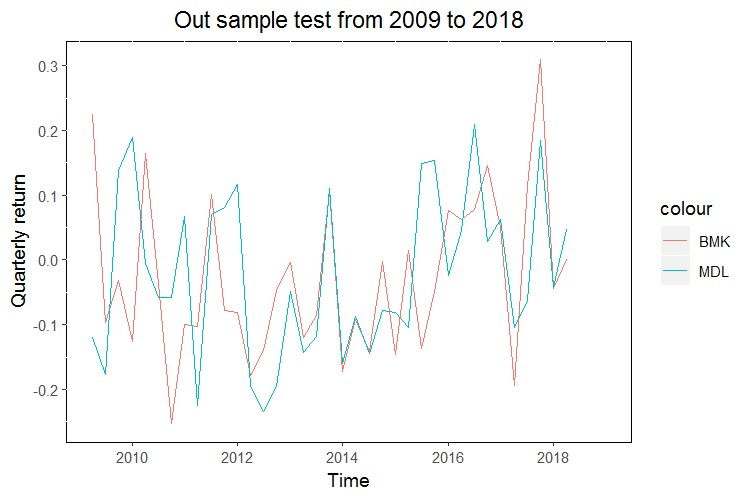
\includegraphics[width=5in]{Lab//full_model.jpg}
\caption{Out of sample quarterly return of technical factor model}
\label{figure16}
\end{center}
\end{figure}

\begin{figure}[H]
\begin{center}
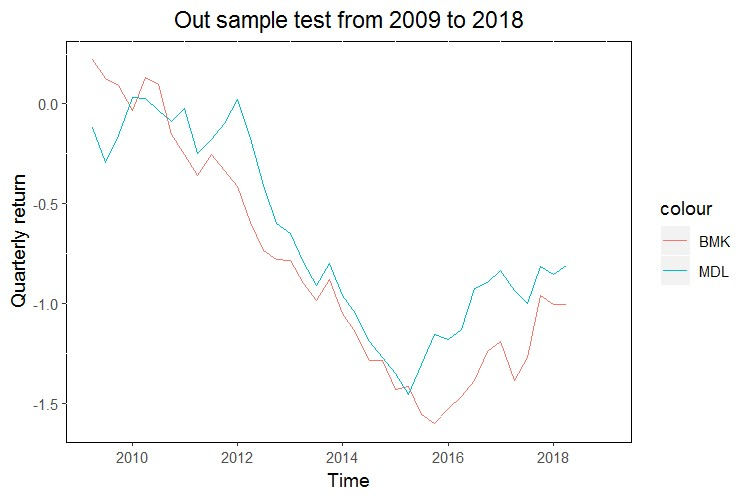
\includegraphics[width=5in]{Lab//full_model_cumu.jpg}
\caption{Out of sample cumulative return of technical factor model}
\label{figure17}
\end{center}
\end{figure}

As we can see, though we are getting negative return, technical factor
model itself improves the performance of the portfolio selected by
fundamental factor model.

\hypertarget{conclusion}{%
\subsubsection{Conclusion}\label{conclusion}}

In this project, we get the following conclusions:

\begin{enumerate}
\def\labelenumi{\arabic{enumi}.}
\item
  Fundamental factor model could generate good information ratio.
\item
  Fundamental factor model suits in bear market, i.e., it would be with
  low risk meanwhile with low return.
\item
  Technical factor model does improve the performance of portfolio
  constructed based on fundamental factor model.
\end{enumerate}

Another thing needs to be mentioned is, though offical fundamental data
would only be released two quarters later than referring quarter, the
performance of companies in referring quarter could be analyzed based on
other information sources in market. Thus, there would be late
efficiency effect if we keep using two quarters' earlier fundamental
factors to predict current quarter's performance.

\hypertarget{references}{%
\subsubsection{References}\label{references}}

\begin{enumerate}
\def\labelenumi{\arabic{enumi}.}
\item
  Kaplan, I., 2014. Value Factors Do Not Forecast Returns for S\&P 500
  Stocks. Available at SSRN 2407303.
\item
  Bohl, L., 2017. Stock Forecasting Fundamental Technical Factors.
\item
  Zephyr. Information Ratio Retrieved from
  \url{http://www.styleadvisor.com/resources/statfacts/information-ratio}
\end{enumerate}


\end{document}
